\documentclass[11pt]{beamer}
\usetheme{CambridgeUS}
\usepackage[utf8]{inputenc}
\usepackage{amsmath}
\usepackage{amsfonts}
\usepackage{amssymb}
\usepackage{graphicx}
\usepackage{pgfpages}
\usepackage{framed}
\usepackage{xcolor}
\usepackage[most]{tcolorbox}
\usepackage{soul}
\usepackage{empheq}
\usepackage{minted}

% The replacement character � (often displayed as a black rhombus with a white
% question mark) is a symbol found in the Unicode standard at code point U
% +FFFD in the Specials table. It is used to indicate problems when a system 
% is unable to render a stream of data to a correct symbol.[4] It is usually 
% seen when the data is invalid and does not match any character. For this 
% reason we map explicitly this character to a blanck space.
\DeclareUnicodeCharacter{FFFD}{ }

\newcommand*{\itemimg}[1]{%
  \raisebox{-.3\baselineskip}{%
    \includegraphics[
      height=\baselineskip,
      width=\baselineskip,
      keepaspectratio,
    ]{#1}%
  }%
}

\newtcbox{\mymath}[1][]{%
    nobeforeafter, math upper, tcbox raise base,
    enhanced, colframe=blue!30!black,
    colback=blue!10, boxrule=1pt,
    #1}

\newcommand{\highlight}[1]{%
  \colorbox{yellow!50}{$\displaystyle#1$}}

\author{Giovanni Della Lunga\\{\footnotesize giovanni.dellalunga@unibo.it}}
%\title{2.1 - Data Pre-Processing}
%\title{4.1 - Linear and Logistic Regression}
%\title{4.2 - Decision Trees}
%\title{Deep Learning Derivatives Pricing}
\title{4 - Introduction to Reinforcement Learning}
\subtitle{} % (optional)
\setbeamercovered{transparent} 
\institute{Advanced Machine Learning for Finance} 
\date{Bologna - April-May, 2022} 

\begin{document}

%\begin{frame}
%\includegraphics[width=\linewidth]{img/halloween-seminar-logo.PNG}
%\end{frame}

\begin{frame}
\titlepage
\end{frame}

\AtBeginSection[]
{
  %\begin{frame}<beamer>
  %\footnotesize	
  %\frametitle{Outline}
  %\begin{multicols}{2}
  %\tableofcontents[currentsection]
  %\end{multicols}	  
  %\normalsize
  %\end{frame}
  \begin{frame}
  \vfill
  \centering
  \begin{beamercolorbox}[sep=8pt,center,shadow=true,rounded=true]{title}  	\usebeamerfont{title}\insertsectionhead\par%
  \end{beamercolorbox}
  \vfill
  \end{frame}
}
\AtBeginSubsection{\frame{\subsectionpage}}

% INSERT HERE

%---------------------------------------------------------------------------------
\section{Basic Ideas}
%---------------------------------------------------------------------------------
\begin{frame}{Reinforcement Learning}
	\begin{itemize}
		\item Some situations by their nature involve a series of decisions rather than a single one. 
		\item Furthermore, as the decisions are taken, the environment may be changing. 
		\item It is then necessary to determine the best action bearing in mind that further decisions have to be taken later
		\item Reinforcement learning is the branch of machine learning that deals with this type of sequential decision making.
		\item The algorithm receives rewards when outcomes are good and incurs costs (negative rewards) when they are bad. 
		\item The objective of the algorithm is to maximize expected future rewards possibly with discounting.
	\end{itemize}
\end{frame}
%..................................................................
\begin{frame}{Reinforcement Learning}
	\begin{itemize}
		\item Basic idea:
		\item Receive feedback in the form of rewards
		\item Agent utility is defined by the reward function
		\item Must (learn to) act so as to maximize expected rewards
	\end{itemize}
	\begin{center}
	\includegraphics[scale=0.5]{../5-pictures/sample_pic_0.png}
	\end{center}
\end{frame}
%..................................................................
\begin{frame}{Reinforcement Learning}
\begin{columns}[T] % align columns
\begin{column}{.48\textwidth}
        \begin{itemize}
		\item \textbf{Supervised Learning}:
		\item Goal: $f(x)=y$
		\item Data: $\left\{ (x_1,y_1);\dots;(x_n,y_n)\right\}$
		\item \textbf{Reinforcement Learning}:
		\item Goal:$$\text{Maximize} \sum\limits_{i=1}^\infty \, \text{Reward}(\text{State}_i, \text{Action}_i)$$
		\item Data: $\text{Reward}_i$,$\text{State}_{i+1}$,$\text{State}_i$, $\text{Action}_i$
        \end{itemize}
\end{column}%
\hfill%
\begin{column}{.48\textwidth}
    %\fbox{
        \includegraphics[width=\linewidth]{../5-pictures/sample_pic_1.png}
    %}
\end{column}%
\end{columns}
\end{frame}
%..................................................................
\begin{frame}{Policy}
	\begin{itemize}
		\item A policy is a mapping from the perceived states of the environment to actions to be taken when in those states
		\item A reinforcement learning agent uses a policy to select actions given the current environment state
	\end{itemize}
	\begin{center}
	\includegraphics[scale=0.6]{../5-pictures/sample_pic_2.png}
	\end{center}
\end{frame}
%..................................................................
\begin{frame}{Reward Signal}
\begin{columns}[T] % align columns
\begin{column}{.48\textwidth}
        \begin{itemize}
		\item The reward signal defines the goal
		\item On each time step, the environment sends a single number called the reward to the reinforcement learning agent
		\item The agent objective is to maximize the total reward that it receives over the long run
		\item The reward signal is used to alter the policy
        \end{itemize}
\end{column}%
\hfill%
\begin{column}{.48\textwidth}
    %\fbox{
        \includegraphics[width=\linewidth]{../5-pictures/sample_pic_3.png}
    %}
\end{column}%
\end{columns}
\end{frame}
%---------------------------------------------------------------------------------
\section{The Multi-armed Bandit Problem}
%---------------------------------------------------------------------------------
%..................................................................
\begin{frame}{A Simple example: K-armed bandits}
\begin{columns}[T] % align columns
\begin{column}{.48\textwidth}
        \begin{itemize}
		\item This is like a one-armed bandit except that you have to choose between $K$ levers.
		\item Lever $k$ provides a return from a normal distribution with mean $m_k$  and standard deviation $1$
		\item Objective is to maximize return over a large number of trials
        \end{itemize}
\end{column}%
\hfill%
\begin{column}{.48\textwidth}
    %\fbox{
        \includegraphics[width=\linewidth]{../5-pictures/chapter-5_pic_0.png}
    %}
\end{column}%
\end{columns}
\end{frame}
\begin{frame}{Strategy}
\begin{columns}[T] % align columns
\begin{column}{.48\textwidth}
        \begin{itemize}
		\item You keep records of the average return from choosing each lever
		\item At each turn you have to decide between
		\item Choose the lever that has given you the best average return so far (the \textit{greedy action})
		\item Try out a new action
        \end{itemize}
\end{column}%
\hfill%
\begin{column}{.48\textwidth}
    %\fbox{
        \includegraphics[width=\linewidth]{../5-pictures/chapter-5_pic_1.png}
    %}
\end{column}%
\end{columns}
\end{frame}
\begin{frame}{Strategy}
\begin{columns}[T] % align columns
\begin{column}{.48\textwidth}
        \begin{itemize}
		\item The first choice is \textbf{exploitation}; the second is \textbf{exploration}.
		\item Exploitation maximizes the immediate expected return but exploration may do better in the long run
        \end{itemize}
\end{column}%
\hfill%
\begin{column}{.48\textwidth}
    %\fbox{
        \includegraphics[width=\linewidth]{../5-pictures/chapter-5_pic_2.png}
    %}
\end{column}%
\end{columns}
\end{frame}
\begin{frame}{Strategy}
\begin{columns}[T] % align columns
\begin{column}{.48\textwidth}
        \begin{itemize}
		\item A strategy for the gambler is to:
		\item Randomly choose a lever with probability $\epsilon$
		\item Choose the lever that has given the best average payoff so far with probability $1-\epsilon$
        \end{itemize}
\end{column}%
\hfill%
\begin{column}{.48\textwidth}
    %\fbox{
        \includegraphics[width=\linewidth]{../5-pictures/chapter-5_pic_3.png}
    %}
\end{column}%
\end{columns}
\end{frame}
\begin{frame}{Strategy}
\begin{columns}[T] % align columns
\begin{column}{.48\textwidth}
        \begin{itemize}
		\item We can implement this strategy by sampling a random number between 0 and 1. If it is less than $\epsilon$ the lever is chosen randomly; otherwise, the lever with the best average payoff so far is chosen. 
		\item We might choose a value of $\epsilon$ equal to one initially and then slowly reduce it to zero as data on the payoffs is obtained
        \end{itemize}
\end{column}%
\hfill%
\begin{column}{.48\textwidth}
    %\fbox{
        \includegraphics[width=\linewidth]{../5-pictures/chapter-5_pic_4.png}
    %}
\end{column}%
\end{columns}
\end{frame}
\begin{frame}{The Math}
	\begin{itemize}
		\item Suppose that lever $k$ has been chosen $n-1$ times and the total reward on the $j$th time it is chosen is $R_j$ 
		\item Expected reward is \begin{equation}Q_k^{old}=\frac{1}{n-1}\sum\limits_{j=1}^{n-1}R_j\end{equation} 
		\item If $k$th lever is chosen for the $n$th time and produces a reward $R_n$ \begin{equation}Q_k^{new}=\frac{1}{n}\sum\limits_{i=1}^n R_i = Q_k^{old}+\frac{1}{n}\left(R_n - Q_k^{old} \right) \end{equation}
	\end{itemize}
\end{frame}
%..................................................................
\begin{frame}{Example}
	Table 7.1, 4 bandits ($m_1=1.2$, $m_2=1$, $m_3=0.8$, $m_4=1.4$); $\epsilon = 0.1$
	\begin{center}
	\includegraphics[scale=0.5]{../5-pictures/chapter-5_pic_5.png}
	\end{center}
\end{frame}
%..................................................................
\begin{frame}{The exploration parameter $\epsilon$ and initial values}
	\begin{itemize}
		\item It makes sense to reduce $\epsilon$ over time. For example we can let it decline exponentially
		\item The initial Q-values make a difference. For example if they all set equal to 2 instead of 0 there would be early exploration
		\item If the standard deviation of the payoff is increased, a higher value of $\epsilon$ would be appropriate 
	\end{itemize}
\end{frame}
%---------------------------------------------------------------------------------
\section{Changing Environment}
%---------------------------------------------------------------------------------
%..................................................................
\begin{frame}{The More General Model: Actions and States }
\footnotesize
\begin{itemize}
\item The multi-armed bandit problem provides a simple example of reinforcement
learning. 
\item \textbf{The environment does not change} and so the Q values
are a function only of the action (i.e., the lever chosen). 
\item In a more general situation, there are a number of states and a number of possible actions and we are dealing with a \textbf{changing environment};
\end{itemize}
	\begin{center}
	\includegraphics[scale=0.5]{../5-pictures/chapter-5_pic_6.png}
	\end{center}
\end{frame}
%..................................................................
\begin{frame}{The More General Model: Actions and States }
\footnotesize
\begin{itemize}
\item The decision maker takes an
action, $A_0$, at time zero when the state $S_0$ is known. This results in a reward, $R_1$, at time $1$ and a new state, $S_1$, is encountered. 
\item The decision
maker then takes another action at time $1$ which results in a reward, $R_2$,
at time $2$ and a new state, $S_2$; and so on. 
\item In this more general situation,
the $Q-value$ \textbf{is a function of both the state and the action taken}.
\end{itemize}
	\begin{center}
	\includegraphics[scale=0.5]{../5-pictures/chapter-5_pic_6.png}
	\end{center}
\end{frame}
%..................................................................
\begin{frame}{The More General Model: Actions and States }
\textbf{Agent-Environment Interaction}
	\begin{itemize}
		\item Set of states $\{S\}$
		\item Set of actions $\{A\}$
		\item In the general case we are facing with a changing environment. We assume that we can define state transition probabilities $p(s^\prime \vert s, a)$. This is the probability distribution over the state space given we take action $a$ in state $s$
		\item Reward function $R : S \times A \rightarrow \mathbb{R}$
		\item For simplicity, assume discrete rewards
		\item Finite Markov Decison Process if both S and A are finite
	\end{itemize}
\end{frame}
%..................................................................
\begin{frame}{The More General Model: Actions and States }
\textbf{Agent-Environment Interaction}
	\begin{itemize}
		\item At each time step, the agent implements a stochastic policy or mapping from states to probabilities of selecting each possible action
		\item The policy is denoted $\pi_t$ where $\pi_t(a \vert s)$ is the probability of taking action $a$ when in state $s$
		\item A policy is a stochastic rule by which the agent selects actions as a function of states
		\item Reinforcement learning methods specify how the agent changes its policy using its experience
	\end{itemize}
\end{frame}
%..................................................................
\begin{frame}{The More General Model: Actions and States}
\textbf{State Transition Probabilities}
	\begin{itemize}
		\item Suppose the reward function is discrete and maps from $S \times A \rightarrow W$
		\item The state transition probability or probability of transitioning to state $s^\prime$ given current state $s$ and action $a$ in that state is given by: \begin{equation} p \left( s^\prime \vert s,a \right) = \sum\limits_{r \in W} p \left( s^\prime, r \vert s,a \right)\end{equation}
	\end{itemize}
\textbf{MDP Dynamics}
	\begin{itemize}
		\item Given current state $s$ and action $a$ in that state, the probability of the next state $s^\prime$ and the next reward $r$ is given by: \begin{equation} p\left( s^\prime, r \vert s,a \right) = \text{Pr} \left( S_{t+1}=s^\prime, R_{t+1} = r \vert S_t =s, A_t = a \right)\end{equation}
	\end{itemize}
	
\end{frame}
%..................................................................
\begin{frame}{Value Function}
	\begin{itemize}
		\item Objective could be to maximize the expected value of rewards
		$$G=R_{t+1}+R_{t+2}+R_{t+3}+\dots+R_{t+T}$$
		\item In some cases, particularly when there is a long or infinite horizon, the objective is to maximize the \textbf{expected value of discounted rewards}:
\begin{equation}
G=R_{t+1}+\gamma R_{t+2}+ \gamma^2R_{t+3}+\dots = \sum\limits_{k=0}^{T-t+1} \gamma^k R_{t+k+1}
\end{equation}
		where $\gamma$ is a discount factor $\le 1$
	\item For each state we have to calculate an utility value equal to the sum of future discounted rewards.	
	\end{itemize}
\end{frame}
%..................................................................
\begin{frame}{Value Function}
	\begin{itemize}
		\item The value of a state is the total amount of reward an agent can expect to accumulate over the future, starting in that state
		\item Compute the value using the states that are likely to follow the current state and the rewards available in those states
		\item Use the values to make and evaluate decisions
		\item Action choices are made based on value judgements
	\end{itemize}
\end{frame}
%..................................................................
\begin{frame}{Value Function}
	\begin{itemize}
		\item Prefer actions that bring about states of \textbf{highest value instead of highest reward}
		\item Rewards are given directly by the environment
		\item Values must continually be re-estimated from the sequence of observations that an agent makes over its lifetime
	\end{itemize}
	\begin{tcolorbox}
	The reward signal indicates what is good in the short run while the value function indicates what is good in the long run
	\end{tcolorbox}
\end{frame}
%..................................................................
\begin{frame}{State-Value Function}
	\begin{itemize}
		\item Value functions are defined with respect to particular policies because future rewards depend on the agent actions
		\item Value functions give the expected return of a particular policy
		\item The value $v_\pi(s)$ of a state $s$ under a policy $\pi$ is the expected return when starting in state $s$ and following the policy $\pi$ from that state onwards
		\begin{align}v_\pi(s) &= \mathbb{E}_\pi \left[G_t \vert S_t=s \right]\notag\\ &= \mathbb{E}_\pi \left[\sum\limits_{k=0}^{T-t-1}\, \gamma^k R_{t+k+1} \vert S_t=s \right]
		\end{align}
\item This is called also \textbf{state-value function}
	\end{itemize}
\end{frame}
%..................................................................
\begin{frame}{Action-Value Function}
	\begin{itemize}
		\item The value $q_\pi(s, a)$ of taking action $a$ in state $s$ under a policy $\pi$  is defined as the expected return starting from $s$, taking the action a and thereafter following policy $\pi$ 
		\item $q_\pi(s,a)$ is the \textbf{action-value function} for policy $\pi$ \begin{align}q_\pi(s,a) &= \mathbb{E}_\pi \left[G_t \vert S_t=s, A_t=a \right]\notag\\ &= \mathbb{E}_\pi \left[\sum\limits_{k=0}^{T-t-1}\, \gamma^k R_{t+k+1} \vert S_t=s , A_t=a \right]
		\end{align}
	\end{itemize}
\end{frame}
%..................................................................
\begin{frame}{Bellman Equation}
For any policy $\pi$ and any state $s$, the following consistency
condition holds between the value of s and the value of its possible successor
states:
\begin{align*}v_\pi(s) &= \mathbb{E}_\pi \left[G_t \vert S_t=s \right] \\ &= \mathbb{E}_\pi \left[\sum\limits_{k=0}^\infty\, \gamma^k R_{t+k+1} \vert S_t=s \right] \\
&= \mathbb{E}_\pi \left[R_{t+1} + \gamma \sum\limits_{n=0}^\infty\, \gamma^n R_{t+n+2} \vert S_t=s \right] \\
&= \sum\limits_a \pi(a,s) \sum\limits_{s^\prime r} p(s^\prime, r \vert s, a)
\left[ r + \gamma \mathbb{E}_\pi \left[ \sum\limits_{n=0}^\infty\, \gamma^n R_{t+n+2} \vert S_{t+1}=s^\prime \right]\right]  \\
&= \sum\limits_a \pi(a,s) \sum\limits_{s^\prime r} p(s^\prime, r \vert s, a)
\left[ r + \gamma  v_\pi(s^\prime)\right]
\end{align*}

\end{frame}
%..................................................................
\begin{frame}{Temporal difference learning}
	\begin{itemize}
		\item So $r +\gamma v_\pi(s^\prime)$ is an unbiased estimate for $v_pi(s)$. 
		\item This observation motivates the following algorithm for estimating $v_\pi(s)$

\item The algorithm starts by initializing a table $V(s)$ arbitrarily, with one value for each state of the MDP. A positive learning rate $\alpha$  is chosen.

\item We then repeatedly evaluate the policy $\pi$ , obtain a reward $r$ and update the value function for the old state using the rule:
\begin{tcolorbox}
\begin{equation} V(S_t) \leftarrow V(S_t) + \alpha \left[ R_{t+1} + \gamma V(S_{t+1}) - V(S_t) \right] \end{equation}
\end{tcolorbox}
	\end{itemize}
\end{frame}
%..................................................................
%---------------------------------------------------------------------------------
\section{A Worked Example: Hedging Portfolio}
%---------------------------------------------------------------------------------
\begin{frame}{RL Application: Hedging}
	\begin{itemize}
		\item Suppose we do not know how to calculate delta
		\item Can reinforcement hedging find a good hedging strategy?
	\end{itemize}
\end{frame}
%..................................................................
\begin{frame}{The set up }
	\begin{itemize}
		\item We want to hedge the sale of 10 call options where $S = 100, K = 100, r = 0, q = 0, \sigma= .2$, and $T = 10$ days or $0.04$ years (we assume 250 trading days in a year).
		\item The hedge is accomplished by owning $0, 1, 2,\dots, 10$ shares (i.e., \textbf{there are 11 possible positions}). 
		\item If the hedger knew that the option would be exercised because the final price of the stock was certain to be greater than 100, it would be optimal for her to buy 10 shares. Similarly, if the hedger knew that the option would be not be exercised because the final price of the stock was certain to be less than 100, it would be optimal for the hedger to hold no shares. 
		\item In practice of course, the outcome is uncertain and, when each hedging decision is made, the hedger \textbf{must choose a position between 0 and 10 shares}.
	\end{itemize}
\end{frame}
%..................................................................
\begin{frame}{The set up }
\textbf{Dynamics}
	\begin{itemize}
		\item We assume that the behavior of the stock price is that the underlying process follows the Black-Scholes-Merton model.
		\item We assume that the hedge position (i.e., number of shares owned) can be changed once a day so that \textbf{a total of 10 decisions have to be made}.
\end{itemize}
\textbf{State}
\begin{itemize}
		\item The states for the reinforcement learning algorithm at the time hedging decision is made on a day and are defined by
		\item \textbf{The number of shares currently held (i.e., the position taken on the previous day)}
		\item \textbf{The stock price}
	\end{itemize}
\end{frame}
%..................................................................
\begin{frame}{The set up }
\textbf{Actions}
	\begin{itemize}
		\item As mentioned there are 11 possible values for the number of shares currently held. 
		\item A total of 15 possible price states are considered:$$\le93, 94, 95, 96, 97, 98, 99, 100, 101, 102, 103, 104, 105, 106, \ge107$$
		\item To simplify matters we assume that \textbf{at most five shares can be bought and five shares can be sold}. 
		\item For example, if the current holding is 7, possible actions (i.e., changes in the position) are -5, -4, -3, -2, -1, 0, +1, +2, and +3. Similarly, if the current holding is 2, possible actions are -2, -1, 0, +1, +2, +3, +4, and +5.
	\end{itemize}
\end{frame}
%..................................................................
\begin{frame}{The set up }
\textbf{Objective}
	\begin{itemize}
		\item The objective function is to \textbf{minimize the variance of the hedging cost}. Since $r=0$ this is equivalent to minimize $$\sum\limits_i H_i^2$$
		\item Hedging cost on day i is $$H_i = N_i(S_{i+1}-S_i)-10\cdot (c_{i+1}-c_i)  $$ where $N_i$ is the number of shares held, $S_i$ is the share price      at the beginning of Day $i$ and $c_i$ is the BSM call option price at the beginning of Day $i$
	\end{itemize}
\end{frame}
%..................................................................
\begin{frame}[fragile]
\frametitle{The Training Algorithm}
\footnotesize
	\textbf{Goal:}
	\begin{itemize}
		\item Build a Q-Table with all state-actions pairs
	\end{itemize}
	\textbf{How:}
	\begin{itemize}
		\item Generating artificial scenarios via Montecarlo simulation
	\end{itemize}
\rule{\textwidth}{1pt}
\begin{minted}{python}
# Initiate Q Table with Q-value = 0 for all state-action pairs
# Option Day to Maturity - TIME DIMENSION
M = 10
# Action [from -5 to 5]  - ACTION DIMENSION 
N_ACTION   = 11
# Number of possible positions [from 0 to 10] - STATE DIMENSION 
N_POSITION = 11
# Set number of state for stock price.        - STATE DIMENSION 
# Prices are round to the nearest integer. Prices >= 107 are assumed to be the same state, Prices <= 93 are assumed to be the same state
STOCK_PRICE_STATE = 15 
q = np.zeros((s.M+1,s.STOCK_PRICE_STATE,s.N_POSITION,s.N_ACTION))
\end{minted}
\rule{\textwidth}{1pt}

\end{frame}
%..................................................................
\begin{frame}[fragile]
\frametitle{The Training Algorithm}
	\textbf{Montecarlo Simulation}
	\begin{itemize}
		\item  TRAINING\textunderscore SAMPLE is the number of simulated path
		\item  Each path contains M time step (days to option maturity)
		\item  Remember, we allow 1 Action per Day 
	\end{itemize}
	\textbf{Output:}	
	\begin{itemize}
		\item price\textunderscore table (2D array) - asset price for each date for each simulation;
		\item call\textunderscore price\textunderscore table (2D array) - call option price for each date for each simulation
		\item delta\textunderscore table - not used in this phase 
	\end{itemize}
\end{frame}
%..................................................................
\begin{frame}[fragile]
\frametitle{The Training Algorithm}
\scriptsize
	\begin{itemize}
		\item Brownian Simulation Function
	\end{itemize}

\rule{\textwidth}{1pt}
\begin{minted}{python}

def brownian_sim(num_path, num_period, mu, std, init_p, dt):
    z = np.random.normal(size=(num_path, num_period))

    a_price = np.zeros((num_path, num_period))
    a_price[:, 0] = init_p

    for t in range(num_period - 1):
        #print(t)
        a_price[:, t+1] = a_price[:, t] * np.exp(
            (mu - (std ** 2) / 2) * dt + std * np.sqrt(dt) * z[:, t]
        )
    return a_price

\end{minted}
\rule{\textwidth}{1pt}
\end{frame}
%..................................................................
\begin{frame}[fragile]
\frametitle{The Training Algorithm}
\scriptsize
	\begin{itemize}
		\item Option Pricing Function
	\end{itemize}

\rule{\textwidth}{1pt}
\begin{minted}{python}

# Function for Black-Scholes Call Option Pricing & Black-Scholes Delta calculation
# T is time to maturity in year
def bs_call(v, T, S, K, r, q):
    np.seterr(divide='ignore', invalid='ignore')
    d1 = (np.log(S / K) + (r - q + v * v / 2) * T) / (v * np.sqrt(T))
    d2 = d1 - v * np.sqrt(T)
    bs_price = S * np.exp(-q * T) * norm.cdf(d1) 
             - K * np.exp(-r * T) * norm.cdf(d2)
    bs_delta = np.exp(-q * T) * norm.cdf(d1)
    return bs_price, bs_delta

\end{minted}
\rule{\textwidth}{1pt}
\end{frame}
%..................................................................
\begin{frame}[fragile]
\frametitle{The Training Algorithm}
\scriptsize
\textbf{Pseudocode for training phase}
\rule{\textwidth}{1pt}
\begin{minted}{python}
epsilon = 1
for k in range(TRAINING_SAMPLE):
	for t in range(DAYS_TO_MATURITY):
		if random <= epsilon:
			# EXPLORATION
			-> choose a random action
		else: 
	    	# EXPLOITATION
	    	-> choose action corresponding to the higher expected value
	    	which in this example is the minimum variance of pnl
		-> Compute Reward - Reward is calculated as expected variance 
			of total pnl from Hedging
    -> Update Q table according to the Temporal Difference Learning Rule 
    Q_NEW = R * Q[t+1]
    Q     = Q + ALPHA*[Q_NEW - Q]
    -> Decrease epsilon to make the agente more likely to exploit   		    
	    			
\end{minted}
\rule{\textwidth}{1pt}
\end{frame}
%..................................................................
\begin{frame}{The Training Algorithm}
	\begin{itemize}
		\item We generated three million paths for the stock price for the training set (the fact that three million paths are necessary for such a small problem emphasizes the point that reinforcement learning is \textit{data hungry}) 
		\item We then used a further 100,000 paths for the test set. 
		\item Initially the \textbf{probability of exploration} was 100\%. 
		\item The probability of exploration decreases as the algorithm proceeds so that the probability of exploration during a trial is 0.999999 times its value at the preceding trial.
		\item The minimum value for the probability of exploration was 5\%.
	\end{itemize}
\end{frame}
%..................................................................
\begin{frame}{Test Set Results}
	\begin{itemize}
		\item The objective was \textbf{to minimize the variance of total hedging costs}
		\item Our results were close to those given by delta hedging
		\item The mean absolute difference between positions taken by the algorithm and those that would be taken with delta hedging when averaged across all hedging days was 0.33
	\end{itemize}
\end{frame}
%..................................................................
\begin{frame}[fragile]
\frametitle{Test Set Results}
\scriptsize
	\begin{itemize}
		\item Pseudocode for Test Program
	\end{itemize}

\rule{\textwidth}{1pt}
\begin{minted}{python}
# Load the Q table from training
q = np.load('Q_RL_Hedging.npy')  
# Asset paths simulation and BS-Parameters calculation for test phase
price_table = brownian_sim(...)
call_price_table, delta_table = bs_call(...)

for i in range(len(price_table)):
    for t in range(DAYS_TO_MATURITY):
        # Position to hold if the agent were to apply delta hedging 
        new_dh_position = bsdelta[t]
        # Get action by finding the minimum non_zero value from the look up table 
        rl_action = np.where(q==min) - 5 
        new_rl_position = rl_action + rl_position 
        rl_reward = (asset[t+1] - asset[t])*new_rl_position 
        - 10*(call[t+1] - call[t])
        dh_reward = (asset[t+1] - asset[t])*new_dh_position 
        - 10*(call[t+1] - call[t])
\end{minted}
\rule{\textwidth}{1pt}
\end{frame}
%..................................................................
\begin{frame}{Test Set Results}
\begin{center}
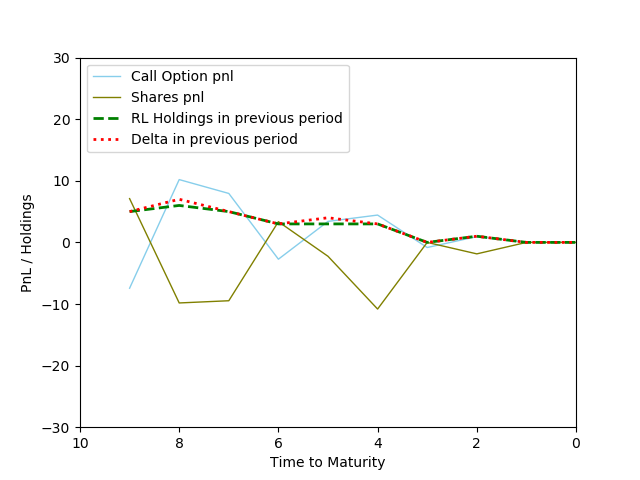
\includegraphics[scale=.6]{../5-pictures/RL-hedge.png} 
\end{center}
\end{frame}
%..................................................................
\begin{frame}{Extension}
	\begin{itemize}
		\item In practice, a trader faces bid-ask spreads, i.e., the ask price at which she or he can buy an instrument is generally higher than the bid price at which she or he can sell the instrument. If bid-ask spreads are not negligible, the trader wants to use a strategy where the cost of buying and selling is weighed against the reduction in risk. 
		\item The objective function can then be $$\sum\limits_i \, \left( C_i + \alpha H_i^2 \right)$$ where $C_i$ is the transaction cost (arising from the bid-ask spread) incurred in period $i$ and $H_i$ is as before the change in the value of the hedger position on day $i$ with the summation being taken over all hedging periods from the current one onward. 
		\item The parameter $\alpha$ defines the trade-off between expected costs and variance of costs.
	\end{itemize}
\end{frame}
%..................................................................
\begin{frame}{Extension}
	\begin{itemize}
		\item Delta hedging is not optimal when transaction costs are considered and the problem is then a genuine multi-period problem that requires reinforcement learning.
		\item The code which accompanies the analysis can be extended to consider this problem
	\end{itemize}
\end{frame}
%..................................................................
%=====================================================================


\end{document}

%..................................................................
\begin{frame}[fragile]
\frametitle{***}
\scriptsize
	\begin{itemize}
		\item ***
	\end{itemize}

\rule{\textwidth}{1pt}
\begin{minted}{python}

% python code

\end{minted}
\rule{\textwidth}{1pt}
\end{frame}
%..................................................................
